\documentclass[a4paper,12pt]{article}

\usepackage{geometry}
\usepackage{polski}
\usepackage{amsmath}
\usepackage{ragged2e}
\usepackage{graphicx}
\usepackage{xcolor}
\usepackage{siunitx}

\graphicspath{ {./images/} }

\newcommand\crule[3][black]{\textcolor{#1}{\rule{#2}{#3}}}

\geometry{
 a4paper,
 total={170mm,257mm},
 left=20mm,
 top=20mm,
 }

\graphicspath{ {./images/} }

\begin{document}
\title{Analiza obrazów - laboratoria 5, 6, 7}
\author{Piotr Moszkowicz} 
\date{\today}
\maketitle
\pagenumbering{roman}

\newpage
\begin{justify}
\tableofcontents
\newpage
\pagenumbering{arabic}

\section{Laboratoria 5}

\paragraph{Na piątych laboratoriach poznawaliśmy operacje morfologiczne, które pozwalają nam na sprawdzenie obiektów, ich relacji względem siebie oraz analizę kształtów na obrazie.}

\begin{figure}[h]
\centering
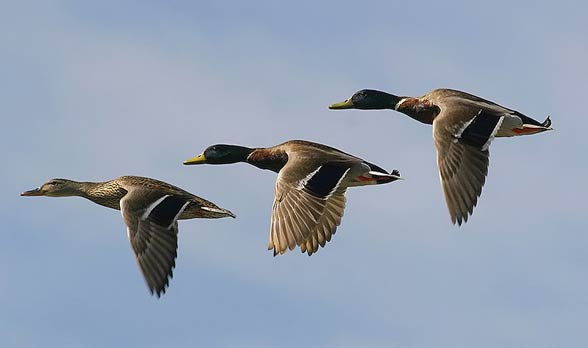
\includegraphics[width=12cm, height=8cm]{kaczki}
\caption{Oryginalny obraz}
\end{figure}

\subsection{Binaryzacja}

\begin{figure}[h]
\centering
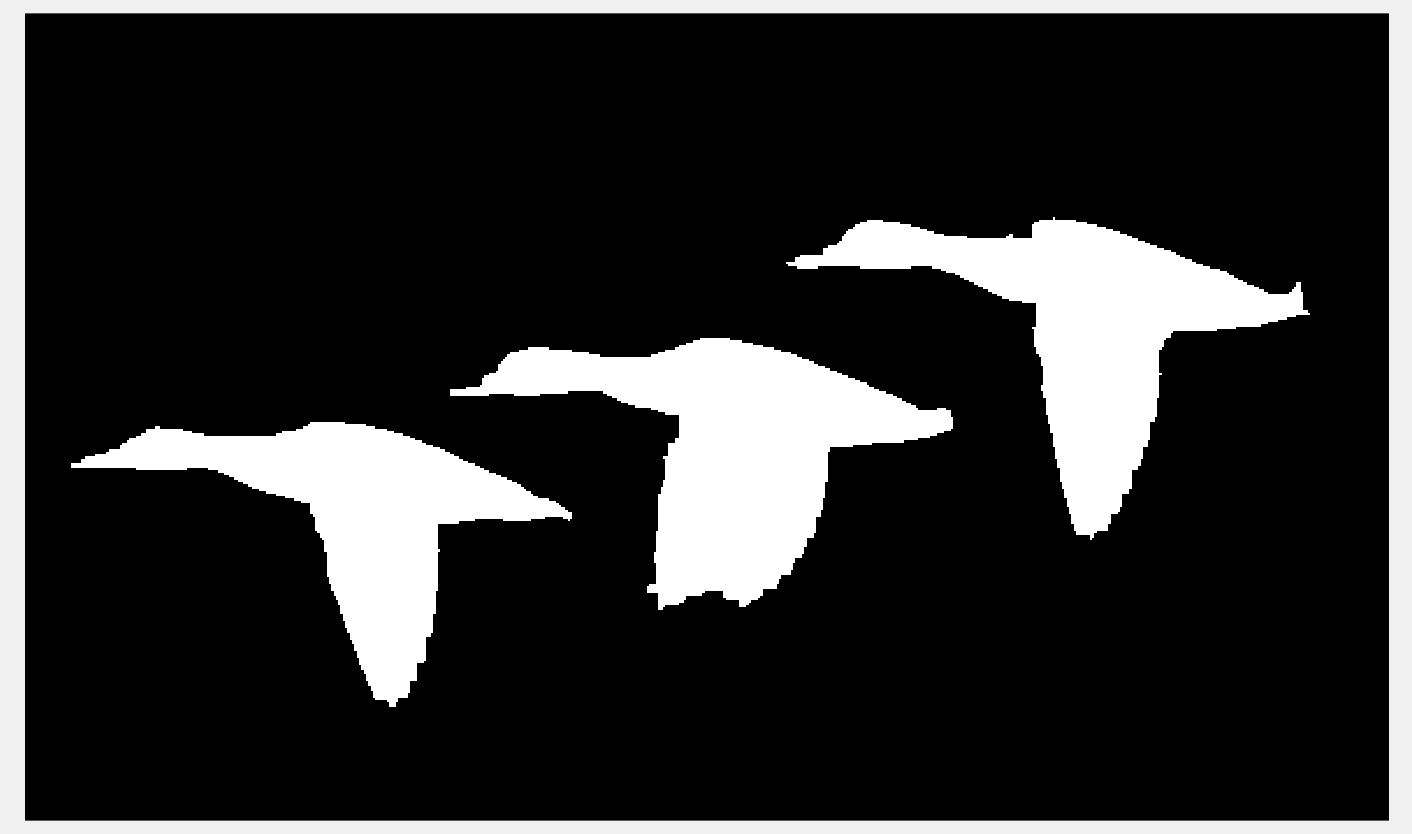
\includegraphics[width=12cm, height=8cm]{1}
\caption{Zbinaryzowany obraz wraz z operacją domknięcia}
\end{figure}

\paragraph{Wszystkie operację przeprowadzamy na zbinaryzowanym, domkniętym obrazie.}

\subsection{Szkieletyzacja obrazu}

\paragraph{Przy pomocy funkcji $bwmorph$ możemy dokonać szkieletyzacji obrazu, dzięki czemu widzimy obiekty przypominające szkielety w naszym wypadku kaczek. Operacja ta polega na wyznaczeniu punktów równoodległych od minimum dwóch krawędzi obiektu. }

\begin{figure}[h]
\centering
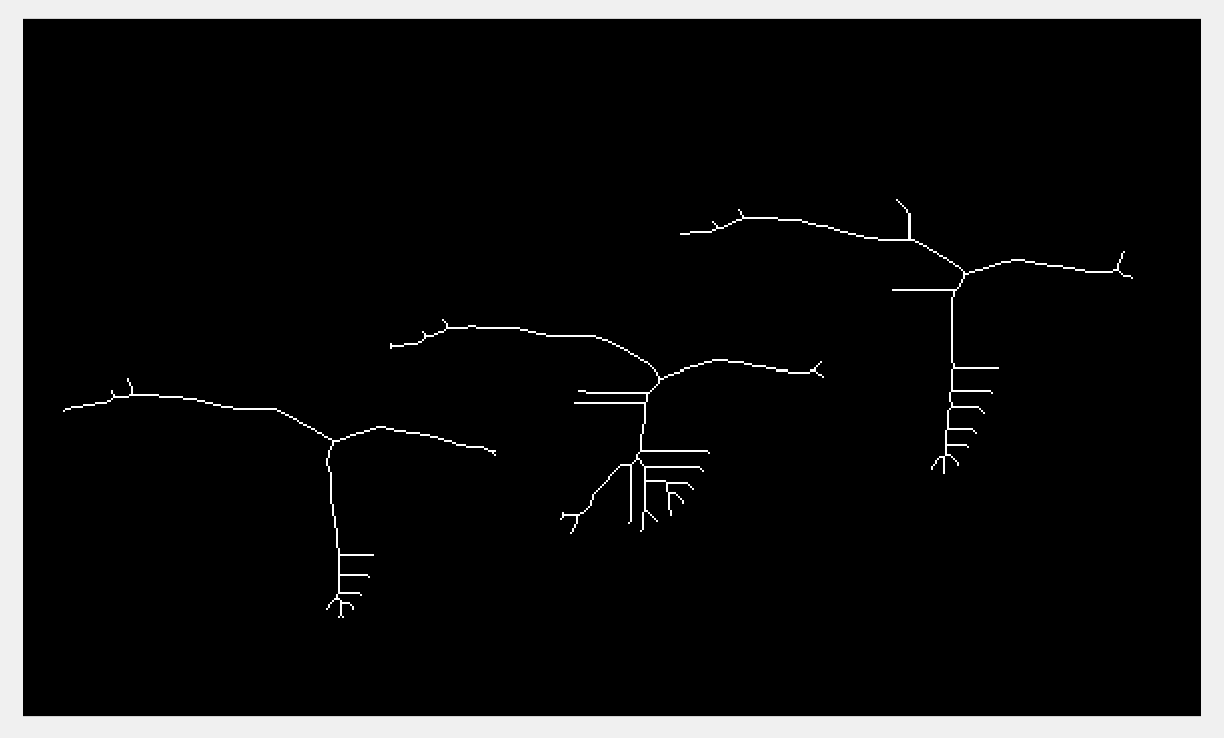
\includegraphics[width=12cm, height=8cm]{2_1}
\caption{Efekt szkieletyzacji}
\end{figure}

\paragraph{Korzystając z tej samej funkcji możemy otrzymać jedynie punkty końcowe szkieletu obrazu.}

\begin{figure}[h]
\centering
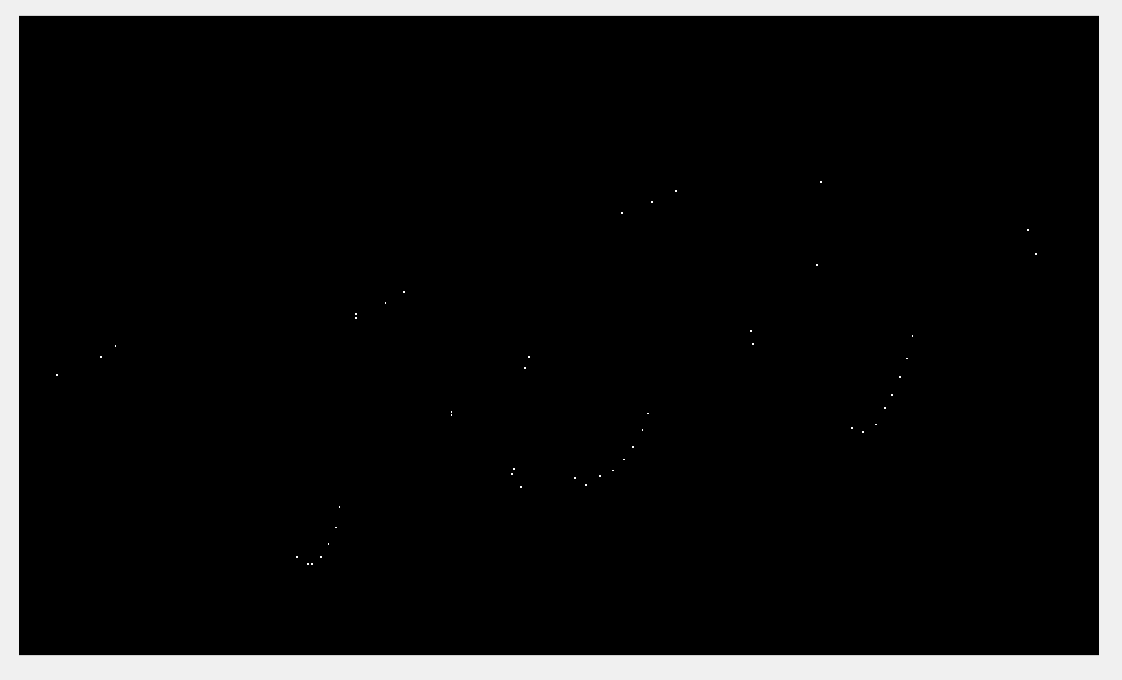
\includegraphics[width=12cm, height=8cm]{2_2}
\caption{Punkty końcowe szkieletu}
\end{figure}

\newpage

\paragraph{Kolejną funkcjonalnością, jaką daje nam $bwmorph$ jest wyznaczenie punktów rozgałęzień szkieletów - one w zupełności wystarczą do oceny orientacji obiektów znajdujących się na obrazie.}

\begin{figure}[h]
\centering
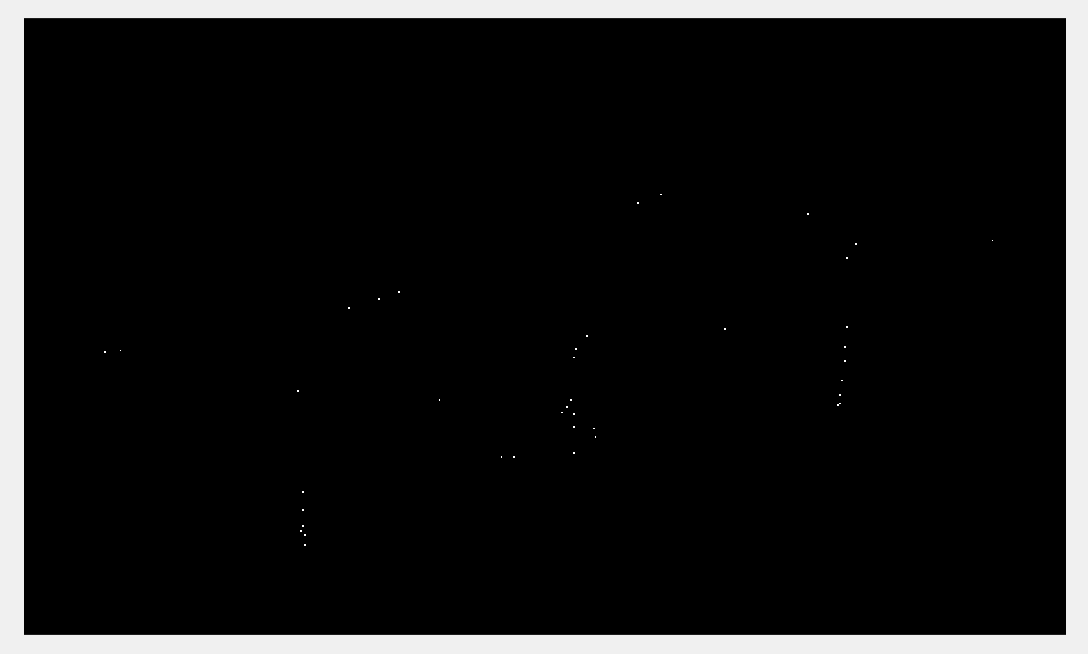
\includegraphics[width=12cm, height=8cm]{2_3}
\caption{Punkty rozgałęzień szkieletu}
\end{figure}

\subsection{Erozja z pomocą $bwmorph$}

\begin{figure}[h]
\centering
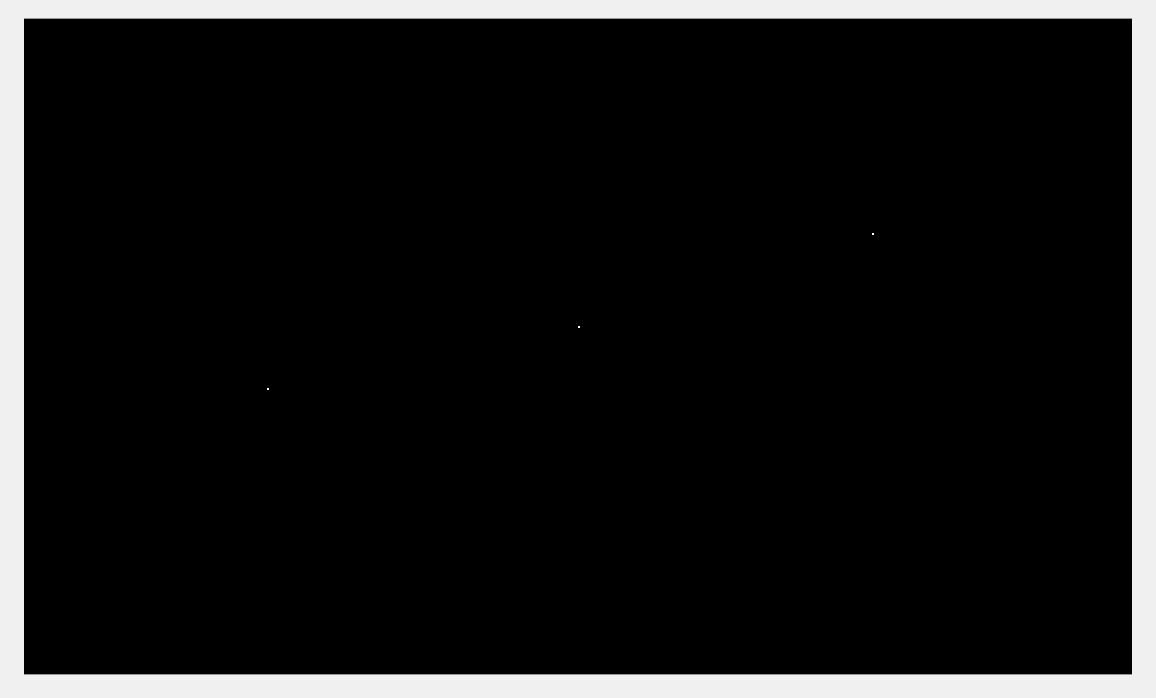
\includegraphics[width=12cm, height=8cm]{3}
\caption{Erozja z argumentem $\infty$}
\end{figure}

\paragraph{Realizacja erozji przy argumencie $\infty$ da nam w efekcie jeden punkt. Warto pamiętać o tym, iż realizacja erozji zachowuje nam liczbę Euler'a. Dzięki temu jesteśmy pewni, że gdy punkt jest samodzielny to nie zostanie on usunięty. }

\newpage

\subsection{Operacja $thin$}

\begin{figure}[h]
\centering
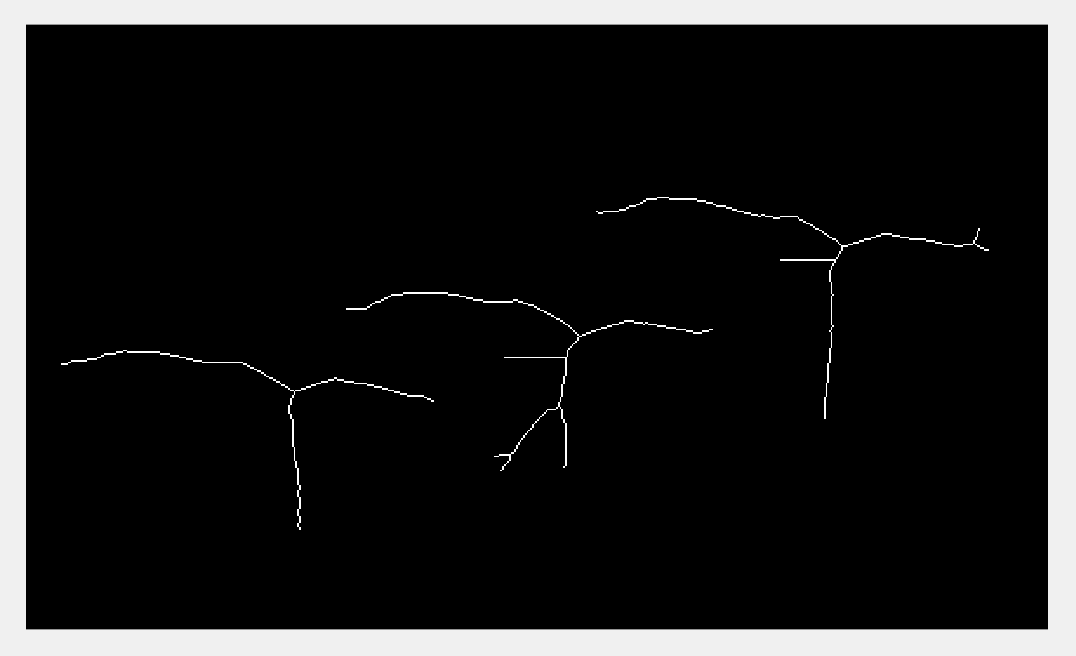
\includegraphics[width=12cm, height=8cm]{4}
\caption{Operacja $thin$ z argumentem $\infty$}
\end{figure}

\paragraph{Operacja $thin$ gwarantuje nam nieusunięcie samodzielnych krawędzi.}

\subsection{Operacja $thicken$}

\begin{figure}[h]
\centering
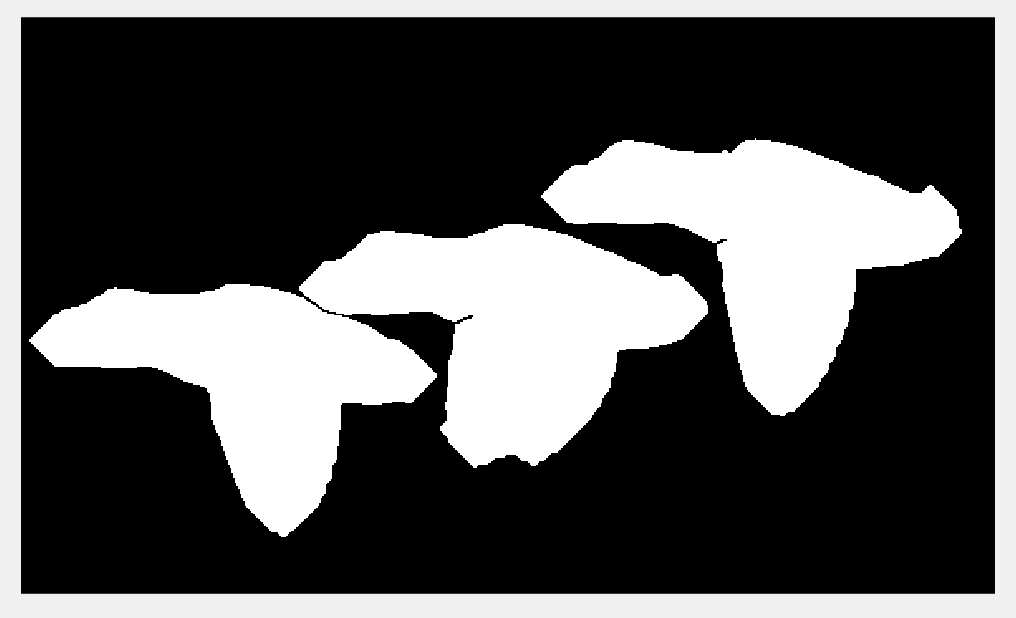
\includegraphics[width=12cm, height=8cm]{5}
\caption{Operacja $thicken$ z argumentem $15$}
\end{figure}

\paragraph{Ta operacja dokonuję dylatację, upewniając się, iż dwa obiekty nigdy się ze sobą nie połączą - tak jak w poprzednich przypadka zachowuje liczbę Euler'a. Każdy biały obszar na obrazie z pewnością zawiera kaczkę i tylko jedną kaczkę.}

\newpage

\subsection{Operacja $remove$}

\begin{figure}[h]
\centering
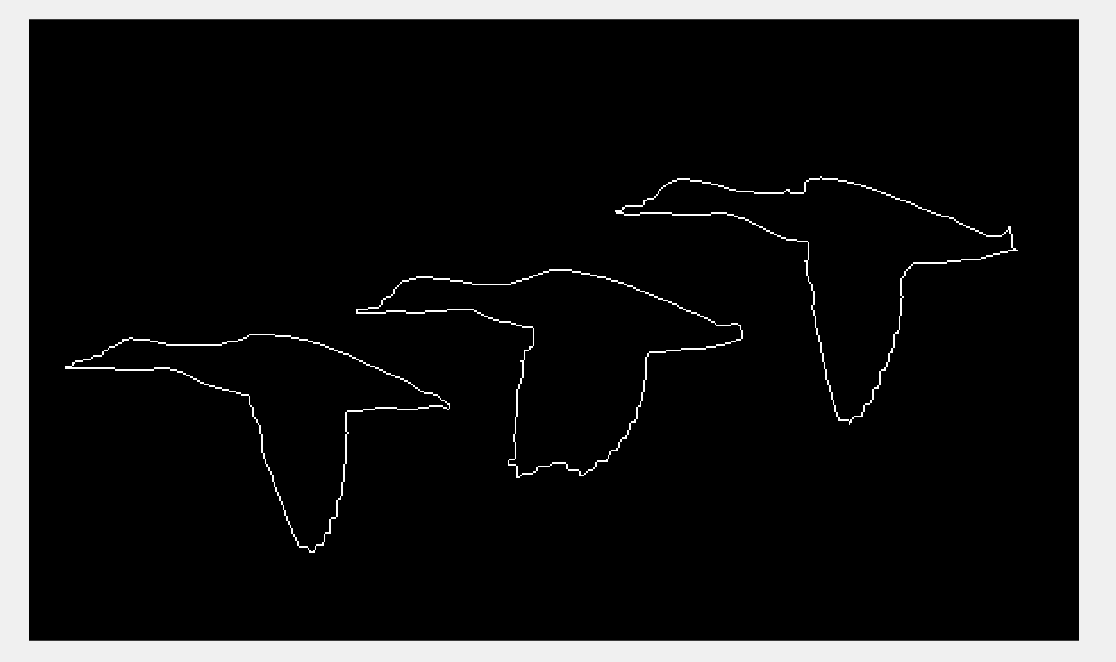
\includegraphics[width=12cm, height=8cm]{6}
\caption{Operacja $remove$ z argumentem $\infty$}
\end{figure}

\paragraph{Operacja $remove$ usuwa wnętrze obiektów - otrzymujemy obraz minus jego erozję.}

\subsection{Segmentacja obrazu}

\begin{figure}[h]
\centering
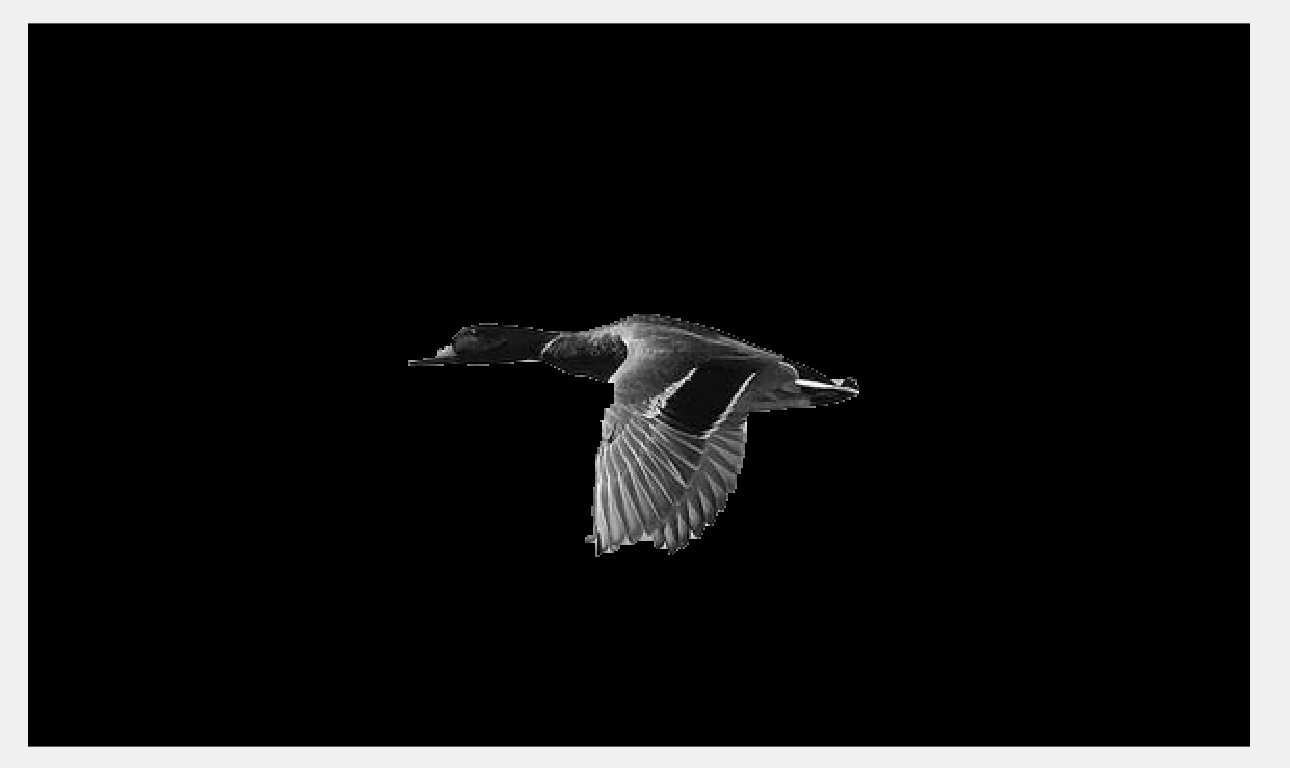
\includegraphics[width=12cm, height=8cm]{7}
\caption{Obraz posegmentowany operacją $bwlabel$ - wyświetlona druga kaczka}
\end{figure}

\paragraph{Segmentacja obrazu pozwala nam oddzielić wszystkie obiekty od siebie - w naszym przypadku otrzymamy tło oraz trzy kaczki. Nadając etykiety białym pikselom upewniamy się, iż ich sąsiedzi mają te same etykiety. Chcąc wyświetlić tło wybralibyśmy etykietę $0$, natomiast etykiety $[1, 3]$ wyświetlą nam kolejne kaczki.}

\newpage

\subsection{Operacja $thicken$ oraz segmentacja}

\begin{figure}[h]
\centering
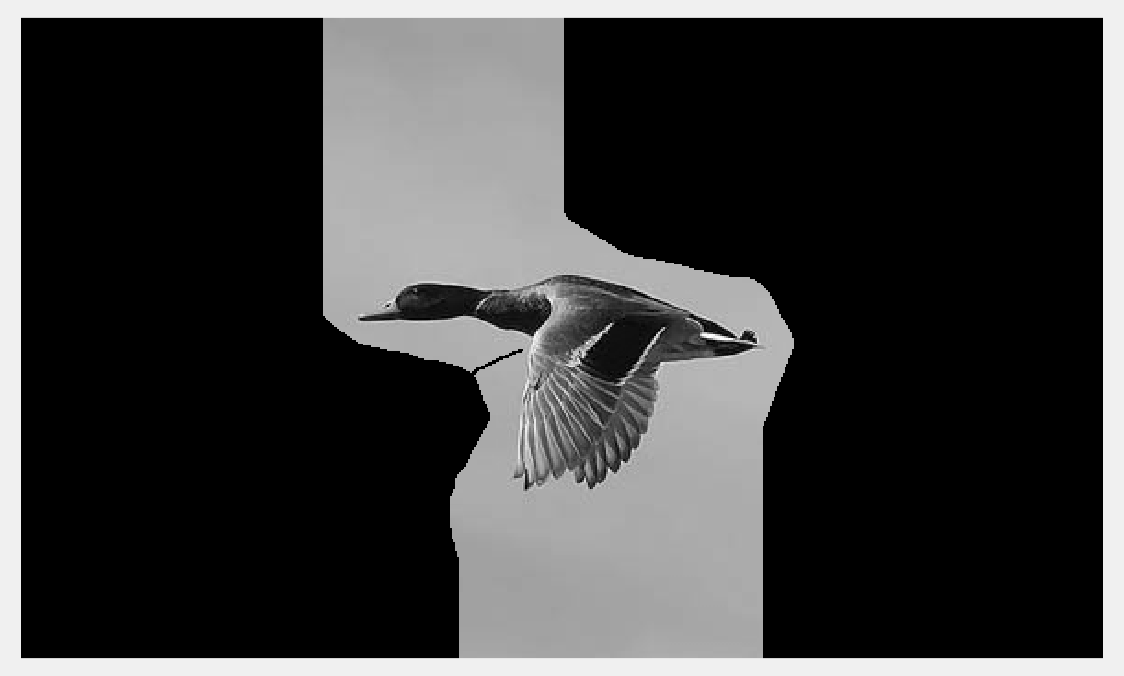
\includegraphics[width=12cm, height=8cm]{8}
\caption{Segment obrazu z drugą kaczką wraz z jej otoczeniem}
\end{figure}

\paragraph{Operacja ta pozwala nam na wyświetlenie danej kaczki wraz z jej otoczeniem.}

\subsection{Jakość segmentacji}

\begin{figure}[h]
\centering
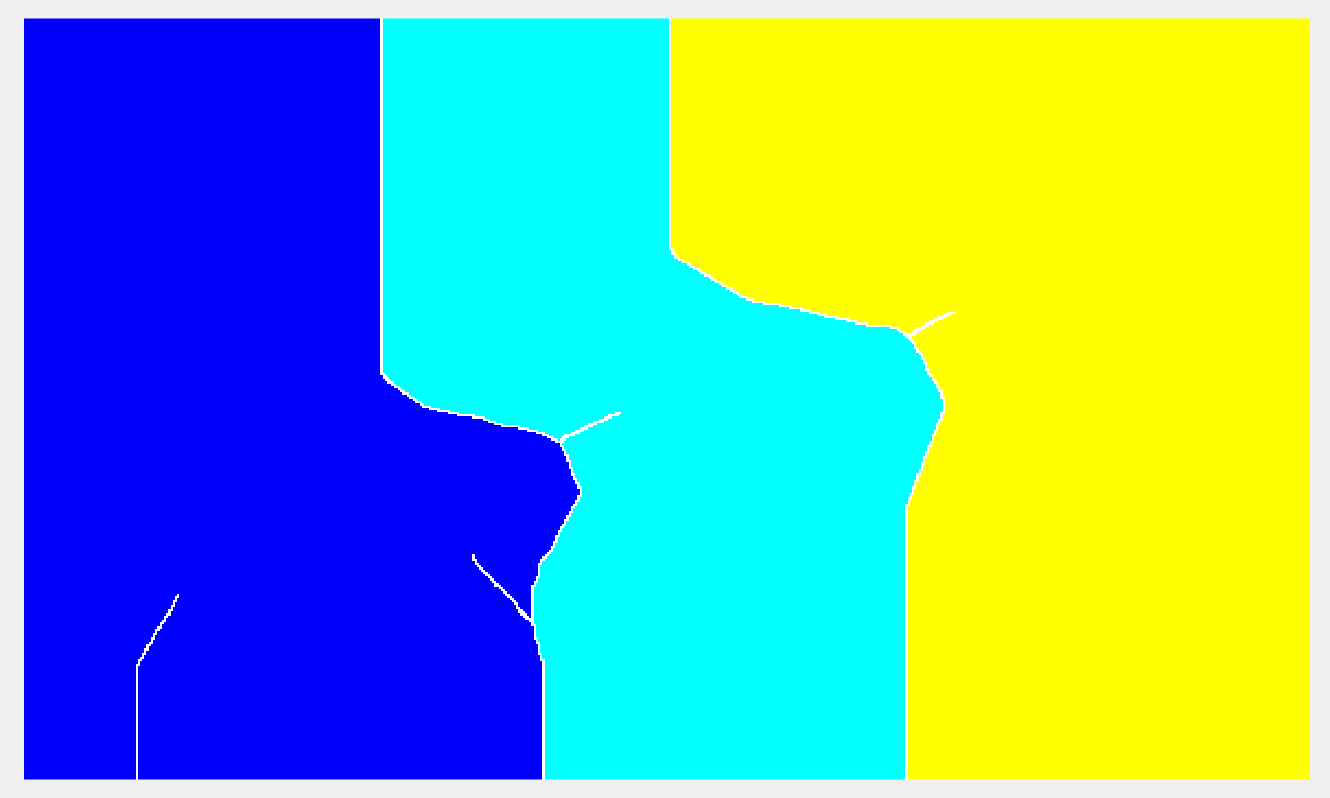
\includegraphics[width=12cm, height=8cm]{9}
\caption{Każdy kolor oznacza inny segment obrazu}
\end{figure}

\paragraph{Możemy również sprawdzać jakość naszej segmentacji - najłatwiejszym sposobem jest oznaczenie każdego segmentu na obrazu osobnym kolorem co widać powyżej.}

\newpage

\subsection{Wododział}

\begin{figure}[h]
\centering
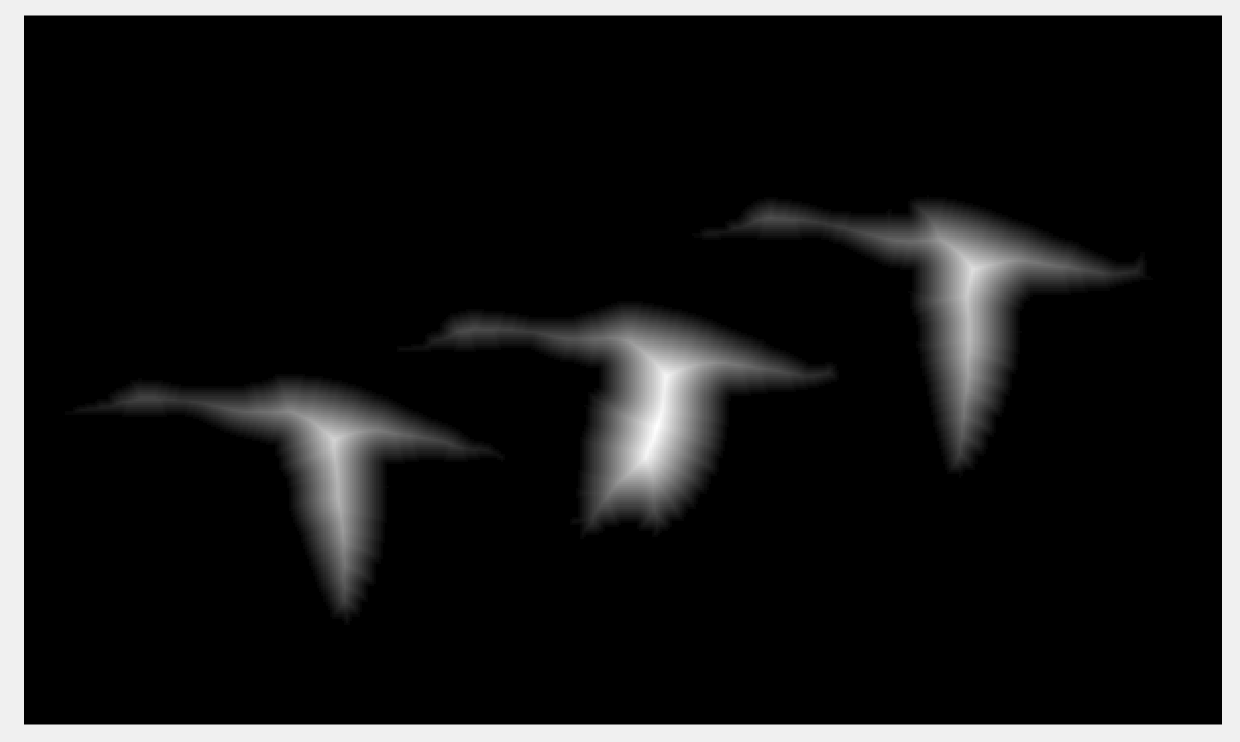
\includegraphics[width=12cm, height=8cm]{10}
\caption{Wododział}
\end{figure}

\paragraph{Wododział - transformata odległościowa obrazu, wpisujemy wartości (w pikselach) odległości od obiektu. Im ciemniejsze punkty, tym dalej znajduje się ten punkt od obiektu.}

\subsection{Segmentacja wododziałowa}

\begin{figure}[h]
\centering
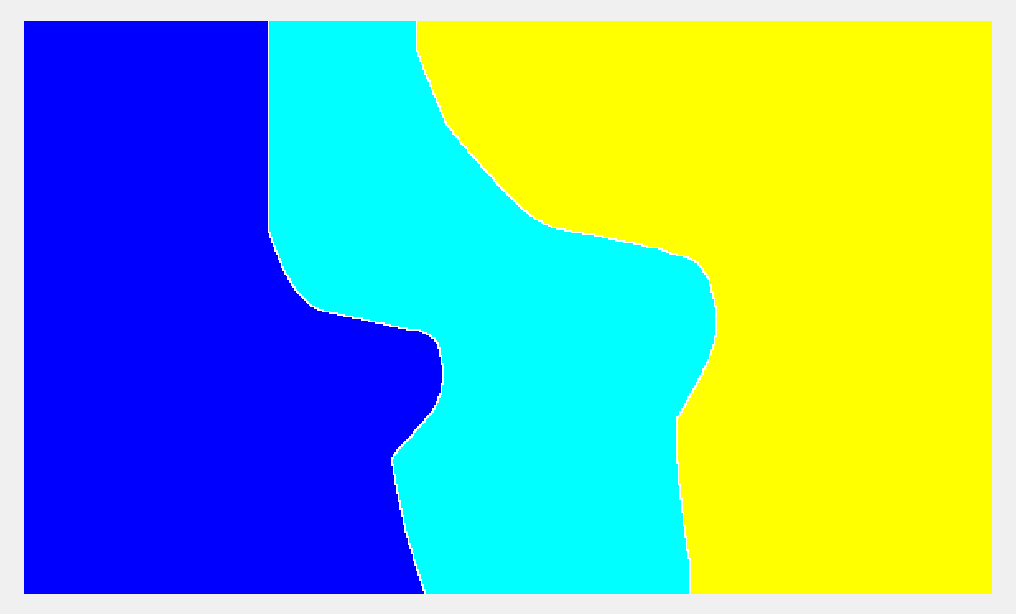
\includegraphics[width=12cm, height=8cm]{11}
\caption{Segmentacja wododziałowa}
\end{figure}

\paragraph{Segmentacja wododziałowa pozwala na dokładniejszą segmentację.}

\newpage

\subsection{Segmentacja wododziałowa z ramką}

\begin{figure}[h]
\centering
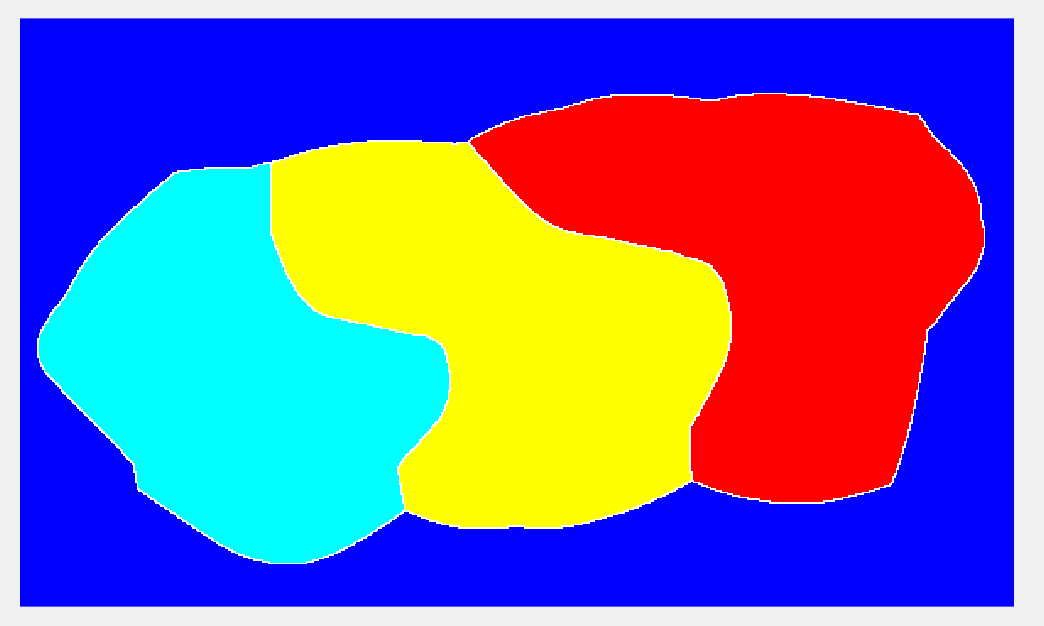
\includegraphics[width=12cm, height=8cm]{12}
\caption{Segmentacja wododziałowa z ramką}
\end{figure}

\paragraph{Segmentacja wododziałowa z ramką wyróżnia nam obiekty od tła.}

\subsection{Segmentacja wododziałowa z metrykami}

\begin{figure}[h]
\centering
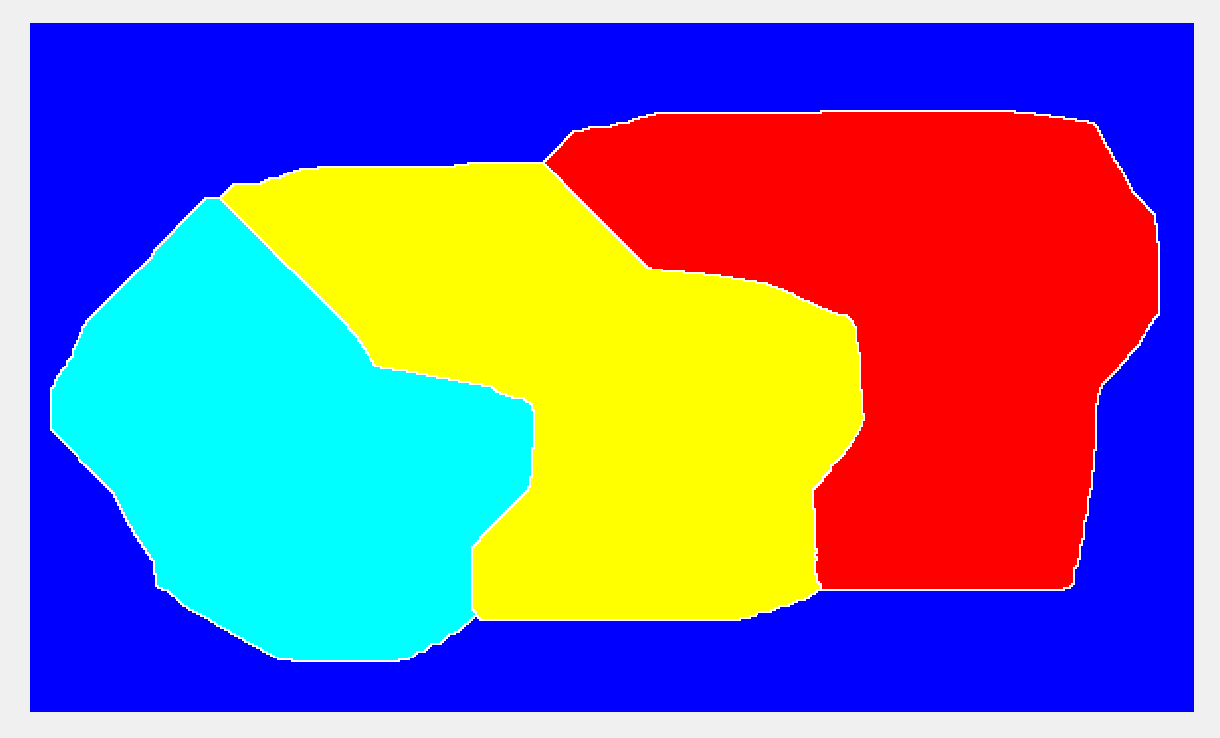
\includegraphics[width=12cm, height=8cm]{13_1}
\caption{Segmentacja wododziałowa z metryką Chebyshev'a}
\end{figure}

\newpage

\begin{figure}[h]
\centering
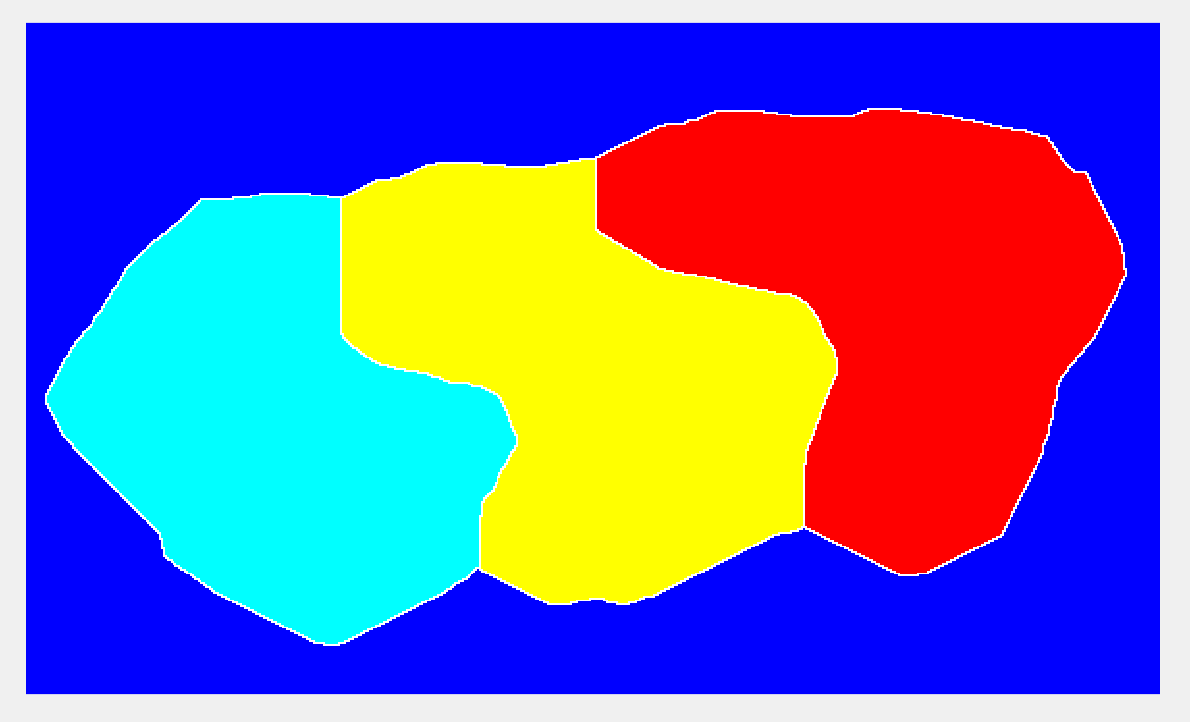
\includegraphics[width=12cm, height=8cm]{13_2}
\caption{Segmentacja wododziałowa z metryką Manhattan}
\end{figure}

\paragraph{Metryki takie jak Chebyshev'a (chessboard) oraz Manhattan (cityblock) pozwalają nam na uzyskanie dokładniejsze segmentacji obrazu.}

\section{Laboratoria 6}

\paragraph{Na szóstych laboratoriach kontynuowaliśmy segmentację, jednak tym razem na podstawie innego obrazka. Tenże obrazek wymagał wyodrębnienia kanałów, aby proces binaryzacji przebiegł pomyślnie.}

\begin{figure}[h]
\centering
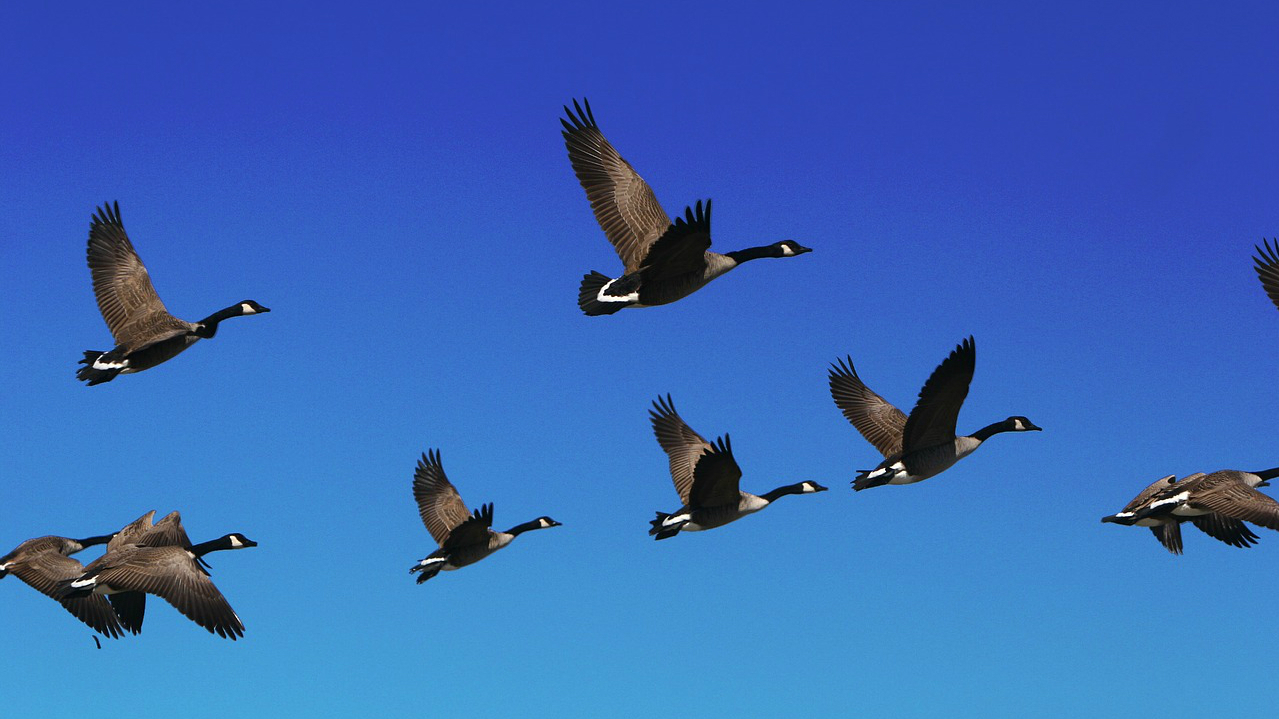
\includegraphics[width=12cm, height=8cm]{ptaki}
\caption{Oryginalny obraz}
\end{figure}

\newpage

\subsection{Segmentacja z wykorzystaniem osobnych kanałów R, G, B}

\begin{figure}[h]
\centering
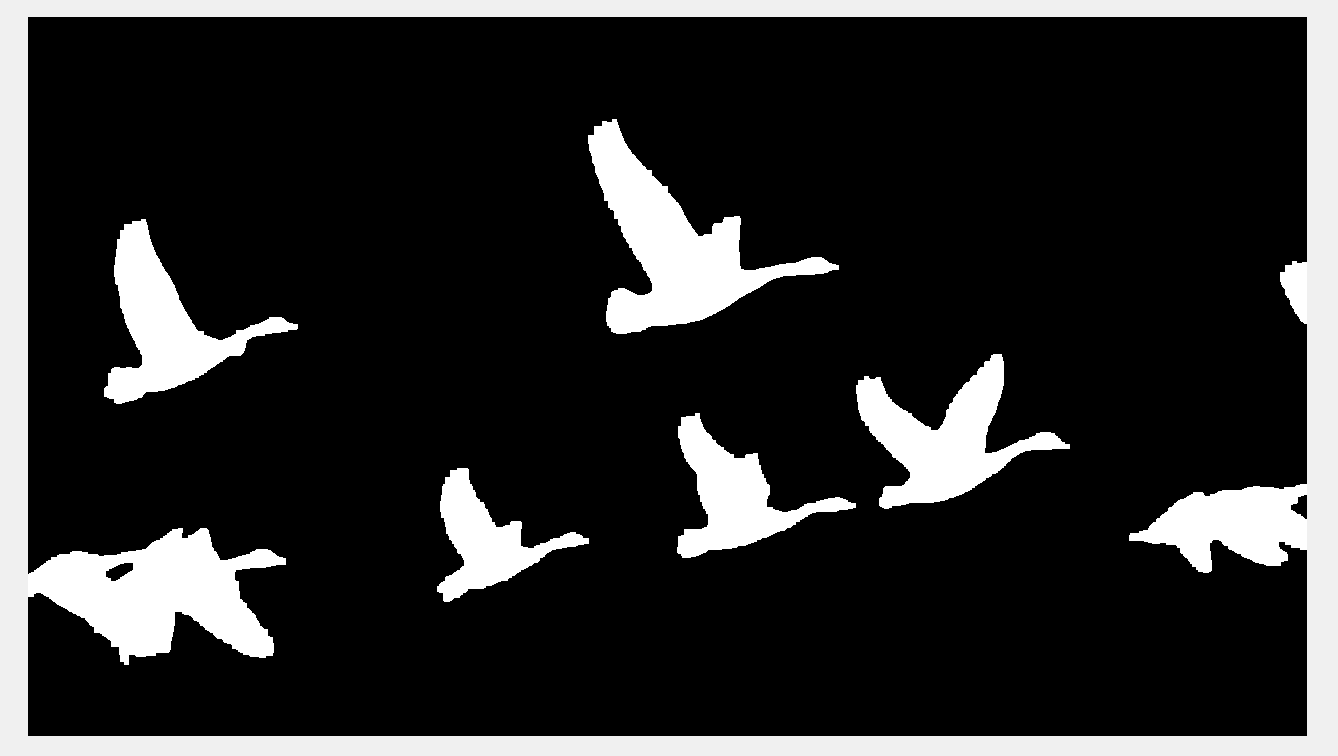
\includegraphics[width=12cm, height=8cm]{14}
\caption{Segmentacja obrazu - binaryzacja kanałów R i B}
\end{figure}

\paragraph{Na podstawie wcześniejszej analizy histogramów zignorowaliśmy kanał G, gdyż wprowadzał za dużo szumów. Dzięki temu w efekcie binaryzacji z domknięciem wyodrębniliśmy obiekty od tła.}

\subsection{Wyznaczanie współczynników poszczególnych kaczek}

\begin{figure}[h]
\centering
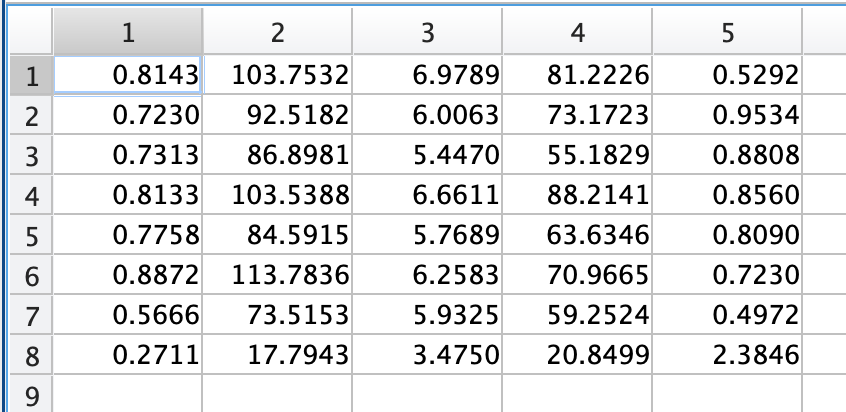
\includegraphics[width=12cm, height=8cm]{15}
\caption{Współczynniki kolejnych kaczek}
\end{figure}

\paragraph{Następnie wyznaczyliśmy różne współczynniki dla każdej z kaczek. Tutaj na obrazku każdy wiersz oznacza kolejne współczynniki dla danej kaczki. Są to kolejno:}

\paragraph{Współczynnik malinowski - podobieństwo figury do koła - 0 -> jest kołem}

\paragraph{Współczynnik Danielsona - średnia odległość piksela od krawędzi,  również podobieństwo figury do koła, również 0 -> jest kołem}

\paragraph{Współczynnika Blair-Bliss'a - średnia odległość piksela od środka masy}

\paragraph{Współczynnik Harlika - odległość piksela na krawędzi od środka masy}

\paragraph{Współczynnik Ferret'a}

\subsection{Metoda 3 sigm - wyznaczanie nietypowych obiektów}

\paragraph{Kolejnym zadaniem, była implementacja metody 3 sigm, która pozwala nam na ocenę podobieństwa danego obiektu do całej reszty. Dzięki temu możemy sprawdzić jakość segmentacji danego segmentu - w tej sytuacji wykryliśmy, iż jako kaczka uznany został kawałek skrzydła.}

\newpage

\section{Laboratoria 7}

\paragraph{Na ostatnich laboratoriach padaliśmy podobieństwo obiektów z pomocą sieci neuronowych. Dzięki temu udało nam się nieskategoryzować wcześniej wspomnianego kawałka skrzydła jako osobnej kaczki.}

\begin{figure}[h]
\centering
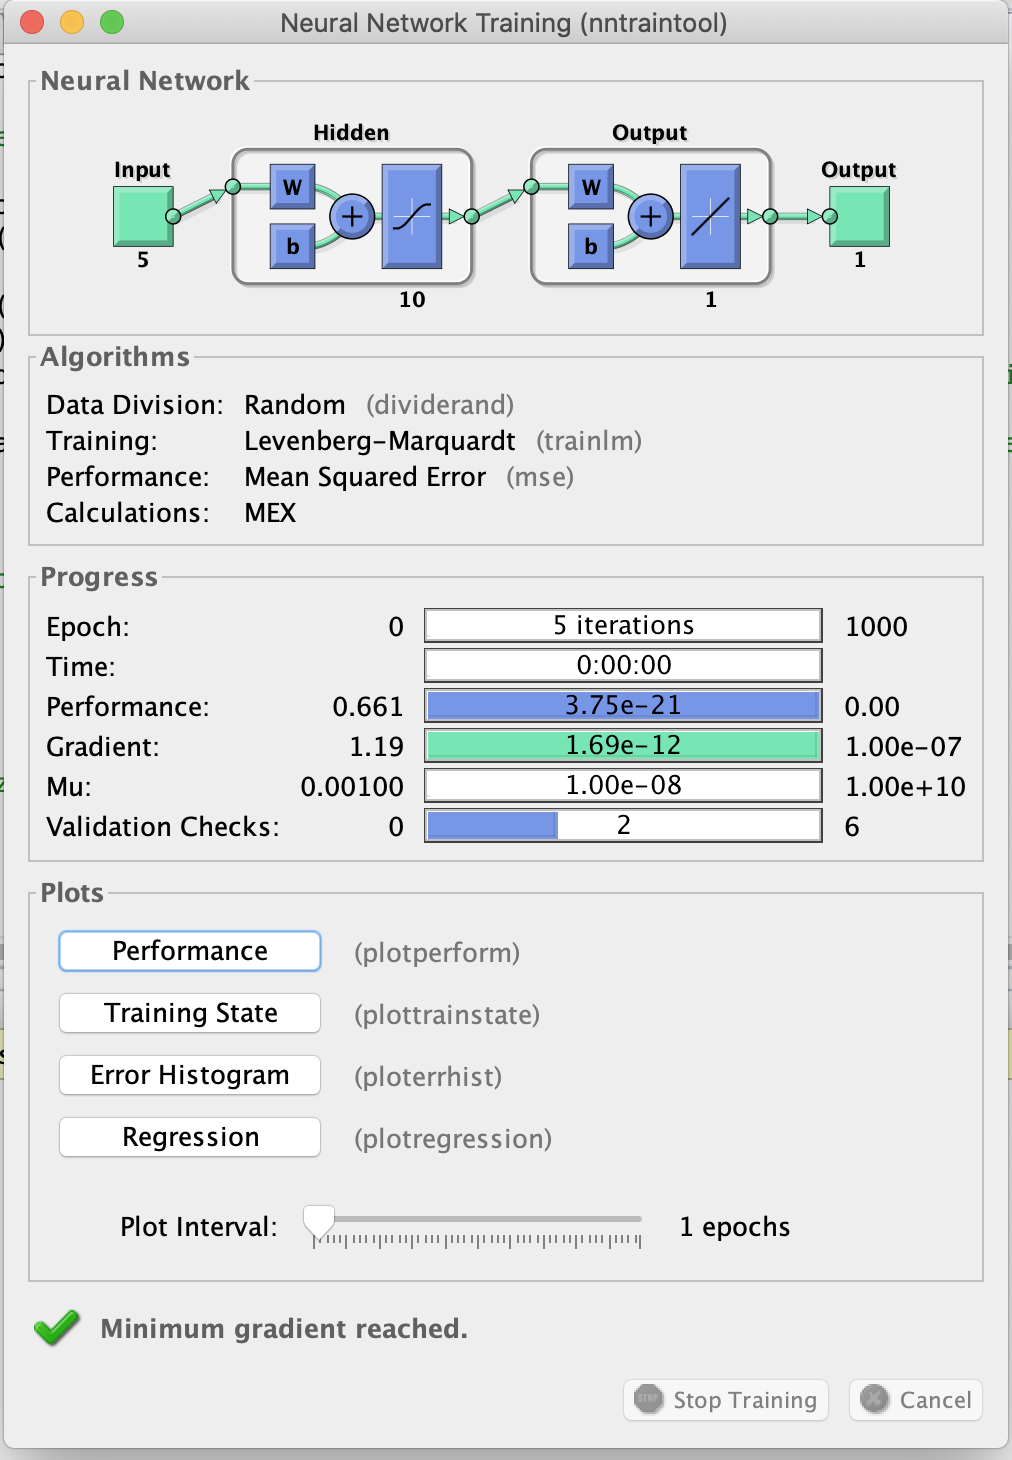
\includegraphics[width=8cm, height=12cm]{16}
\caption{Trening sieci neuronowej w oprogramowaniu Matlab}
\end{figure}

\newpage

\end{justify}
\end{document}